\documentclass{exam}

% Language and font encodings
\usepackage[greek,english]{babel}
\usepackage[utf8x]{inputenc}

% Math
\usepackage{amsmath} % math
\usepackage{amssymb} % symbols
\usepackage{amsthm}
\usepackage{sectsty}
\usepackage{enumitem}

% Table of signs and plots
\usepackage{pgf,tikz}
\usepackage{tkz-tab}
\usetikzlibrary{shapes,snakes,arrows,backgrounds}
\usetikzlibrary{scopes,svg.path,shapes.geometric,shadows}
\usepackage{graphicx}
\usepackage{xcolor}
\usepackage{xpatch}

% Page numbering
\footer{}{\thepage}{}

% grpah functions
\usepackage{pgfplots}

\pgfplotsset{compat=1.10}

\usepgfplotslibrary{fillbetween}

% tkz-tab hardcodes $0$ for the zeros
\xpatchcmd{\tkzTabLine}{$0$}{$\bullet$}{}{}
% we want solid lines
\tikzset{t style/.style={style=solid}}

\renewcommand{\qedsymbol}{$\blacksquare$}

\title{\textgreek{Μια συλλογή σύντομων ασκήσεων στα \\ Μαθηματικά Γ' λυκείου}}
\date{\underline{\textgreek{Λύσεις}}}
\author{\textgreek{Παναγιώτης Πετρίδης}}

\begin{document}
    \maketitle
    \thispagestyle{empty}
    \newpage
    \begin{questions}
        \vspace{1.5cm}
        \setcounter{page}{1}
\setcounter{equation}{0}

\question

\begin{center}
\begin{proof}[\unskip\nopunct]
\begin{align}
    \notag
    &\int_{\alpha}^{\beta}f(x)dx + \int_{\gamma}^{\delta}f^{-1}(x)dx = \beta\cdot\delta - \alpha\cdot\gamma\notag
    \implies \int_{\alpha}^{\beta}f(x)dx + \int_{\gamma}^{\delta}f^{-1}(x)dx = \left[xf(x)\right]_{\alpha}^{\beta}\\
    &\implies \int_{\alpha}^{\beta}f(x)dx = \left[xf(x)\right]_{\alpha}^{\beta} - \int_{\gamma}^{\delta}f^{-1}(x)dx
\end{align}
\textgreek{Θέτοντας $u=f^{-1}(x)\implies x=f(u) \implies dx=f'(u)du$ και $u_1 = f^{-1}(\gamma) = \alpha$, $u_2 = f^{-1}(\delta) = \beta$}
\begin{align}
    \int_{\gamma}^{\delta}f^{-1}(x)dx = \int_{\alpha}^{\beta}uf'(u)du = \int_{\alpha}^{\beta}xf'(x)dx
\end{align}

\textgreek{Οπότε θα έχουμε: }
\begin{align*}
    \underset{\mathrm{(2)}}{\overset{\mathrm{(1)}}{\implies}} \implies \int_{\alpha}^{\beta}f(x)dx = \left[xf(x)\right]_{\alpha}^{\beta} - \int_{\alpha}^{\beta}xf'(x)dx
\end{align*}
\textgreek{Το οποίο ισχύει καθώς είναι ο ορισμός της ολοκλήρωσης κατα παράγοντες.}
\end{proof}

\end{center}

        \vspace{1.5cm}
        \setcounter{equation}{0}

\question 

\begin{align*}
    f(x) = \sqrt{1 - x^2}, x\in[-1,1]
    \implies y = \sqrt{1 - x^2}
    \implies y^2 = 1 - x^2
    \implies y^2 + x^2 = 1, y > 0
\end{align*}

\begin{center}
\textgreek{Άρα η $f$ αποτελεί το πάνω κομμάτι ημικυκλίου\\}

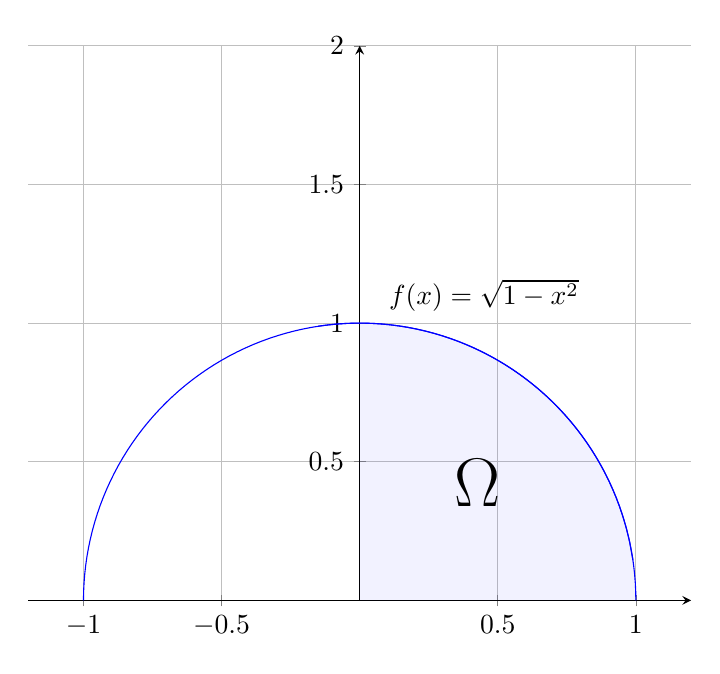
\begin{tikzpicture}
\begin{axis}[
    domain=0:2*pi,samples=100,grid=major,
    width=10cm,
    axis lines = middle,
    xmin=-1.2, xmax=1.2, ymin=0, ymax=2,
]
            
\addplot[color=blue, trig format plots=rad, domain=0:pi] ({cos(x)}, {sin(x)});
\addplot[name path=f,domain=-.15:1.05,blue] {sqrt(1-x^2)};
      
\path[name path=axis] (axis cs:0,0) -- (axis cs:1,0);
    \addplot [
        thick,
        color=blue,
        fill=blue,
        fill opacity=0.05
    ]
    fill between[
        of=f and axis,
        soft clip={domain=0:1},
    ];
    \node [rotate=0] at (axis cs:  .45,  1.1) {$f(x) = \sqrt{1-x^2}$};
    \node [rotate=0] at (axis cs:  .425,  .425) {\Huge$\Omega$};
\end{axis}
\end{tikzpicture}

\textgreek{Άρα ισχύει ότι: }
\begin{equation*}
    E(\Omega) = \frac{\pi\cdot r^2}{4} = \frac{\pi}{4}
\end{equation*}
\end{center}

        \vspace{1.5cm}
        \setcounter{equation}{0}
\question \textgreek{Σωστή απάντηση: $i$}
\begin{proof}[\unskip\nopunct]
\begin{align*}
    &e^\pi > \pi^e\\
    \underset{\mathrm{\pi^e > 0}}{\overset{\mathrm{e^\pi > 0}}{\implies}}& \pi > eln\pi\\
    \implies& \pi - eln\pi > 0
\end{align*}
\begin{center}
\textgreek{Το οποίο ισχύει. Διότι: }
        
\textgreek{Έστω $f(x) = x-elnx$, $x > 0$.}
        
\textgreek{Η $f$ είναι παραγωγήσιμη ως πράξεις παραγωγήσιμων σηναρτήσεων.}
\end{center}
\begin{equation*}
    f'(x) = 1 - \frac{e}{x} = \frac{x-e}{x}, x>0
\end{equation*}
\begin{align*}
    &f'(x) = 0 \implies \frac{x-e}{x} = 0 \implies x = e\\
    &x > e \implies x-e > 0 \overset{x>0}{\implies} \frac{x-e}{x} > 0\\
    &x < e \implies x-e < 0 \overset{x>0}{\implies} \frac{x-e}{x} < 0
\end{align*}

\begin{center}
    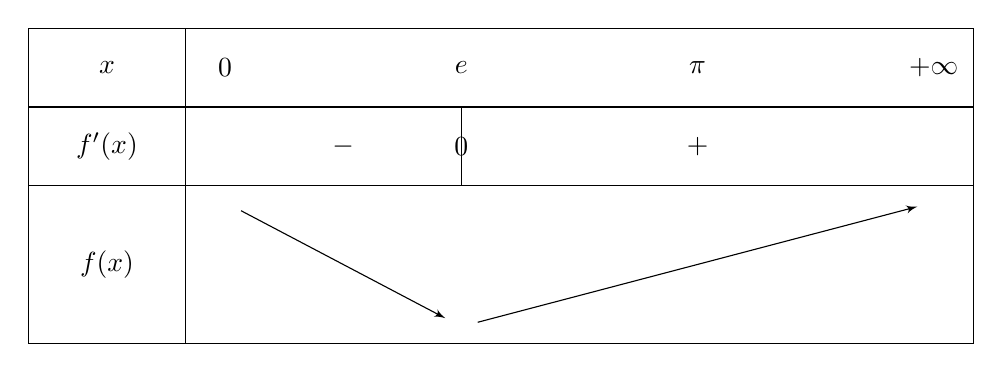
\begin{tikzpicture}
        \tkzTabInit[espcl=3]{$x$ /1,$f'(x)$ /1, $f(x)$ /2 }
            {$0$ ,$e$, $\pi$, $+\infty$}
        \tkzTabLine {,-,z,,+ ,  }
        \tkzTabVar{+/,-/, R/, +/}
    \end{tikzpicture}
\end{center}

\begin{center}
\textgreek{Άρα το $f(e)$ είναι (ολικό) ελάχιστο. Οποτέ θα έχουμε ότι: }
\begin{align*}
    &f(\pi) > f(e)\\
    \implies &\pi - eln\pi > e - elne\\
    \implies &\pi - eln\pi > 0
\end{align*}
\end{center}
\end{proof}

        \vspace{1.5cm}
        \setcounter{equation}{0}

\question \textgreek{Αρχικά έχουμε ότι: }

\begin{center}
        
\begin{align*}
    &\int_{-1}^{1}(1-x)^\kappa dx = \left[\frac{(1-x)^{\kappa+1}}{\kappa+1}\right]_{-1}^{1} = -\frac{2^{\kappa+1}}{\kappa+1}\\
    \implies &\lim_{\kappa\to0}\int_{-1}^{1}(1-x)^\kappa dx = \lim_{\kappa\to0}-\frac{2^{\kappa+1}}{\kappa+1} = \lim_{\kappa\to0}-\frac{2^{\kappa+1}}{\kappa+1}
    = \lim_{\kappa\to0}-\frac{e^{(\kappa+1)ln2}}{\kappa+1}\\
    \overset{\mathrm{u=\kappa+1}}{=\joinrel=\joinrel=} & \lim_{u\to0}-\frac{e^{uln2}}{u} = (-1)\cdot \pm \infty
\end{align*}
        
\textgreek{Άρα το όριο δεν υπάρχει.\\ Παίρνοντας το όριο στο $+\infty$ έχουμε: }
        
\begin{align*}
    \lim_{\kappa\to+\infty}-\frac{2^{\kappa+1}}{\kappa+1} = &\lim_{\kappa\to+\infty}-\frac{2^{\kappa+1}}{\kappa+1}
    = \lim_{\kappa\to+\infty}-\frac{e^{(\kappa+1)ln2}}{\kappa+1}
    \overset{\mathrm{u=\kappa+1}}{=\joinrel=\joinrel=}\lim_{u\to+\infty}-\frac{e^{uln2}}{u}\\
    \underset{\mathrm{DLH}}{\overset{\left(\frac{\infty}{\infty}\right)}{=\joinrel=}}&\lim_{u\to+\infty}-\frac{ln2\cdot e^{uln2}}{1} = -ln2 \cdot (+\infty) = -\infty
\end{align*}
        
\end{center}

        \vspace{1.5cm}
        \setcounter{equation}{0}

\question  

\begin{align*}
    &y^2 - 2y -x^2 + 1 = 0
    \implies y^2 - 2y -x^2 + 1 -x + x = 0\\
    \implies &y^2 - 2y -x^2 + 1 -x + x  -xy + xy = 0\\
    \implies &y^2 +xy -y -xy -x^2 + x -y -x + 1 = 0\\
    \implies &(y-x-1)(y+x-1)=0
\end{align*}
\begin{center}
\textgreek{Οπότε οι ευθείες είναι: $(\varepsilon_1): y = x + 1$ και $(\varepsilon_2): y = -x + 1$}
        
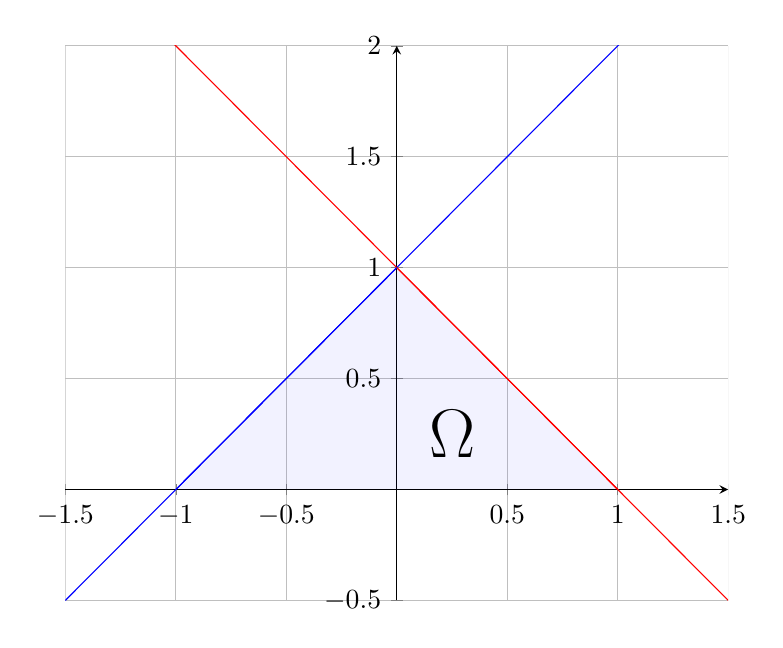
\begin{tikzpicture}
    \begin{axis}[
        samples=100,grid=major,
        width=10cm,
        axis lines = middle,
        xmin=-1.5, xmax=1.5, ymin=-0.5, ymax=2,
    ]
    \addplot[blue] (x,x+1);
    \addplot[red] (x,-x+1);
    \addplot[name path=e1, red, domain=0:1] (x,-x+1);
    \addplot[name path=e2, blue, domain=-1:0] (x,x+1);
    \path[name path=axis] (axis cs:-1,0) -- (axis cs:1,0);
    \addplot [
        thick,
        color=blue,
        fill=blue,
        fill opacity=0.05
    ]
    fill between[
        of=e2 and axis,
        soft clip={domain=-1:1},
    ];
    \node [rotate=0] at (axis cs:  .25,  .25) {\Huge$\Omega$};
    \end{axis}
\end{tikzpicture}
      
\textgreek{Οπότε έχουμε ότι:}
      
\begin{equation*}
    E(\Omega) = \frac{1}{2}2\cdot 1 = 1
\end{equation*}

\end{center}

        \vspace{1.5cm}
        \setcounter{equation}{0}
        
\question  
        
\textgreek{Έχουμε ότι: }
\begin{equation}
    e = \lim_{x\to0}(1+x)^\frac{1}{x}
\end{equation}
\begin{proof}[\unskip\nopunct]

\textgreek{Οπότε: }
\begin{align*}
    &\lim_{h\to0}\frac{ln(x+h) - lnx}{h} = \lim_{h\to0}\frac{ln(\frac{x+h}{x})}{h} = \lim_{h\to0}\frac{1}{h}\cdot ln(1 + \frac{h}{x})\\
    \overset{u=\frac{h}{x}}{=} &\lim_{u\to0}\frac{1}{x\cdot u}\cdot ln(1 + u) = \lim_{u\to0}\frac{1}{x}\cdot ln((1 + u)^\frac{1}{u})\\
    \overset{\mathrm{(1)}}{=} &\frac{1}{x}\cdot lne = \frac{1}{x}
\end{align*}
\end{proof}

        \vspace{1.5cm}
        \setcounter{equation}{0}
        
\question  

\begin{align*}
    f(x) = \varepsilon\varphi x,x\in[0,\frac{\pi}{2})\cup(\frac{\pi}{2}, \frac{3\pi}{2}) && y=\frac{2\sqrt{3}}{7\pi}x
\end{align*}
        
\begin{center}
\textgreek{Για την $f$ έχουμε ότι: }
\begin{align*}
    f(x) = \varepsilon\varphi x,x &\in D_f \implies f'(x) = \frac{1}{\sigma\upsilon\nu^2 x} > 0, \forall x\in D_f\\
    &f''(x) = 2\frac{\varepsilon\varphi x}{\sigma\upsilon\nu^2 x}
\end{align*}

\textgreek{Άρα η $f\uparrow[0,\frac{\pi}{2})=A_1$ και $f\uparrow(\frac{\pi}{2}, \frac{3\pi}{2})=A_2$}
\vspace{3mm}
      
\textgreek{Για $x\in[0,\frac{\pi}{2})$ η $f:$ κυρτή αφού $f''(x)>0$, για $x\in(\frac{\pi}{2}, \pi]$ η $f:$ κοίλη αφού $f''(x)<0$, τέλος για $x\in[\pi, \frac{3\pi}{2})$ η $f:$ κυρτή αφού $f''(x)>0$\\}
      
\vspace{3mm}
\textgreek{Επειδή όμως η εξήσωση της εφαπτομένης της $f$ στο 0 είναι: $y=x$ και η $f$ κυρτή στο $[0,\frac{\pi}{2})$ η $f$ είναι πάνω απο την $y=x$.}
\vspace{3mm}
      
\textgreek{Όμως και $y=\frac{2\sqrt{3}}{7\pi}x < x$ οπότε η $f(x)\geq\frac{2\sqrt{3}}{7\pi}x$, ισότητα μόνο για $x=0$ στο $[0,\frac{\pi}{2})$}
\vspace{3mm}
      
\textgreek{Για $\frac{\pi}{2} < x < \pi$ η $f(x) < 0$ και $\frac{2\sqrt{3}}{7\pi}x > 0$ άρα η $f$ δεν τέμνει την $y = \frac{2\sqrt{3}}{7\pi}x$ στο $(\frac{\pi}{2},\pi]$}
\vspace{3mm}
      
\textgreek{Για $x\in({\pi}, \frac{3\pi}{2})$}
\begin{align*}
    &g(x) = f(x) - \frac{2\sqrt{3}}{7\pi}x = \varepsilon\varphi x - \frac{2\sqrt{3}}{7\pi}x\\
    \implies &g(x) = \varepsilon\varphi x - \frac{2\sqrt{3}}{7\pi}x \implies g(x) = \varepsilon\varphi x -  \frac{\sqrt{3}}{3}\cdot \frac{6}{7\pi}x =  \varepsilon\varphi x - \varepsilon\varphi \left(\frac{7\pi}{6}\right)\cdot \frac{6}{7\pi}x\\
    \implies &g(x) = \varepsilon\varphi x - \varepsilon\varphi \left(\frac{7\pi}{6}\right)\cdot \frac{6}{7\pi}x
\end{align*}
      
\textgreek{και}
      
\begin{equation*}
    g'(x) = \frac{1}{\sigma\upsilon\nu^2 x} - \frac{2\sqrt{3}}{7\pi} > 0, \forall x\in({\pi}, \frac{3\pi}{2})
\end{equation*}
      
\textgreek{Αφού: }
\begin{align*}
    2\sqrt{3} < 2\cdot 3 = 6 \implies 2\sqrt{3} < 6 < 7 \implies \frac{2\sqrt{3}}{7} < 1
\end{align*}
\textgreek{και}
\begin{align*}
    x\in({\pi}, \frac{3\pi}{2}) \implies -1 < \sigma\upsilon\nu x \leq 0 \implies 1 < \sigma\upsilon\nu^2 x \implies \frac{1}{\sigma\upsilon\nu^2 x} > 1
\end{align*}
      
\textgreek{Άρα η $g\uparrow({\pi}, \frac{3\pi}{2})$ και $g(\frac{7\pi}{6}) = 0$ άρα $x=\frac{7\pi}{6}$ μοναδική ρίζα στο $({\pi}, \frac{3\pi}{2})$}
\vspace{3mm}
      
\textgreek{Άρα τελικά $x=0$ και $x=\frac{7\pi}{6}$ μοναδικές ρίζες της εξήσωσης $f(x) = \frac{2\sqrt{3}}{7\pi}x$}
\vspace{3mm}
      
\textgreek{Κάνοντας μια πρόχειρη γραφική παράσταση έχουμε: }
      
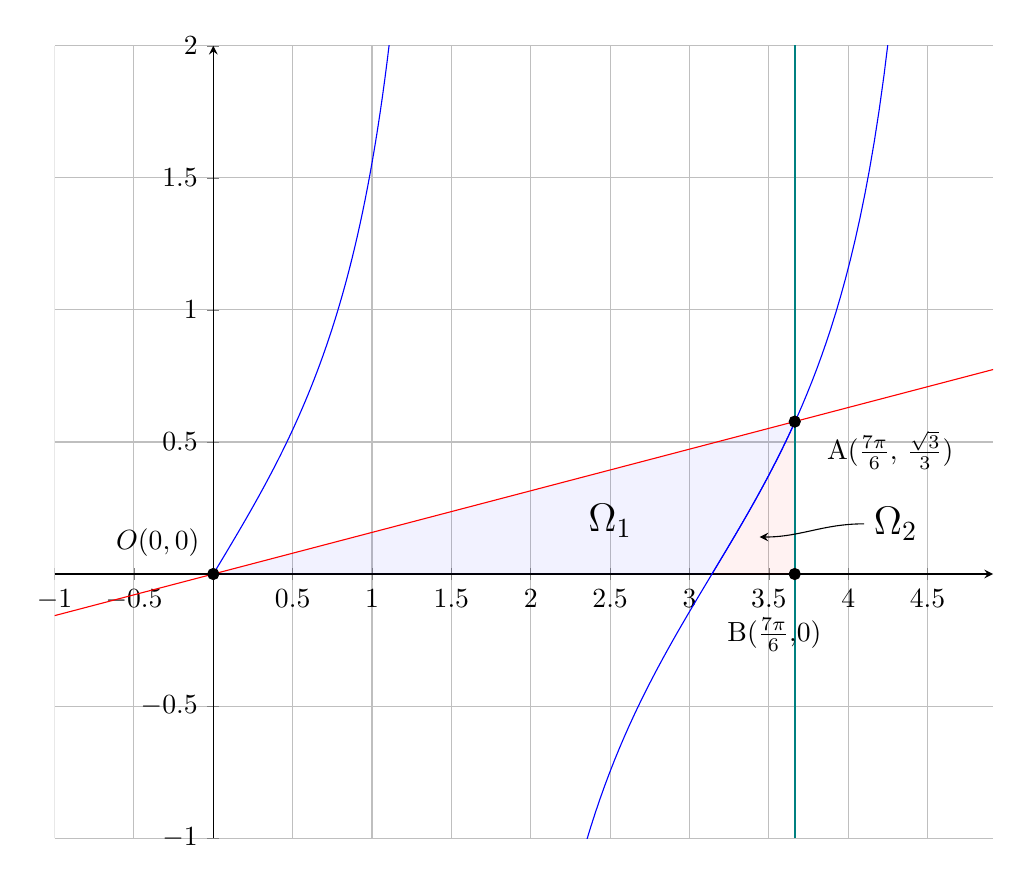
\begin{tikzpicture}
\begin{axis}[
        samples=100,grid=major,
        width=13.5cm,
        axis lines = middle,
        xmin=-1, xmax=3*pi/2+0.2, ymin=-1, ymax=2,
    ]
    \addplot[domain=0:3.1/2, blue] {sin(deg(x))/cos(deg(x))};
    \addplot[domain=3.3/2:(3*3.1)/2, blue] {sin(deg(x))/cos(deg(x))};
    \addplot[name path=t1, domain=pi:7*pi/6, blue] {sin(deg(x))/cos(deg(x))};
      
    \addplot[thick, domain=0:6,teal] coordinates {(7*pi/6,-1)(7*pi/6,3)};
    \addplot[name path=q1, thick, domain=0:6,teal] coordinates {(7*pi/6,0)(7*pi/6,0.5777)};
    
    \path[name path=axis] (axis cs:-1,0) -- (axis cs:4,0);
    \addplot[name path=l1, red] {((2*sqrt(3))/(7*3.14))*x};
    \node [rotate=0] at (axis cs:  7*pi/6+0.6,  0.47) {A($\frac{7\pi}{6}$, $\frac{\sqrt{3}}{3})$};
    \node [rotate=0] at (axis cs:  -0.35,  0.12) {$O(0,0)$};
    \node [rotate=0] at (axis cs:  7*pi/6-0.13,  -0.23) {B($\frac{7\pi}{6}$,0)};
    \addplot [only marks] table {
        0   0
        3.663   0
        3.663   0.577
    };
      
    \addplot [
        thick,
        color=blue,
        fill=blue,
        fill opacity=0.05
    ]
        fill between[
            of=l1 and t1,
            soft clip={domain=0:7*pi/6},
    ];
      
    \addplot [
        thick,
        color=red,
        fill=red,
        fill opacity=0.05
    ]
        fill between[
        of=t1 and q1,
        soft clip={domain=0:4},
    ];
    \node[anchor=west] (source) at (axis cs:4.1,0.19){\Large$\Omega_2$};
    \node (destination) at (axis cs:3.38,0.14){};
    \draw[->,>=stealth](source) to [out=180,in=0] (destination);
    \node [rotate=0] at (axis cs:  2.5,  .2) {\Large$\Omega_1$};
\end{axis}
\end{tikzpicture}

\textgreek{Οπότε έχουμε ότι $E(\Omega_1) = (AOB) - E(\Omega_2)$}
\textgreek{Επειδή η $f$ είναι περιοδική με περίοδο $\pi$ θα ισχύει ότι: }
\begin{align*}
    &E(\Omega_2) = \int_{\pi}^{\frac{7\pi}{6}}f(x)dx = \int_{\pi-\pi}^{\frac{7\pi}{6} - \pi}f(x)dx = \int_{0}^{\frac{\pi}{6}}f(x)dx\\
    \implies &E(\Omega_2) = \int_{0}^{\frac{\pi}{6}}\varepsilon\varphi xdx = \int_{0}^{\frac{\pi}{6}}\frac{\eta\mu x}{\sigma\upsilon\nu x}dx
    \overset{\mathrm{u = \sigma\upsilon\nu x}}{=\joinrel=\joinrel=} \int_{1}^{\frac{\sqrt{3}}{2}}-\frac{(u)'}{u}dx\\
    \implies &E(\Omega_2) = \int_{\frac{\sqrt{3}}{2}}^{1}\frac{(u)'}{u}dx = \Big[lnu\Big]_{\frac{\sqrt{3}}{2}}^{1} = ln1 - ln(\frac{\sqrt{3}}{2}) = - ln(\frac{\sqrt{3}}{2})
\end{align*}
\textgreek{Οπότε τέλος έχουμε ότι: }
\begin{align*}
    E(\Omega_1) = (AOB) &- E(\Omega_2) = \frac{7\pi}{6}\cdot \frac{\sqrt{3}}{3}\cdot\frac{1}{2} - ln(\frac{\sqrt{3}}{2})\\
    \implies &E(\Omega_1) = \frac{7\pi\sqrt{3}}{36} - ln(\frac{\sqrt{3}}{2})
\end{align*}
\end{center}

        \vspace{1.5cm}
        \setcounter{equation}{0}
        
\question  

\textgreek{Έχουμε ότι: }
\begin{center}
\begin{align}
    f(x) = \eta\mu kx \quad x,k>0 \quad x \leq \frac{\pi}{k}
\end{align}
\textgreek{Γραφηκά έχουμε ότι: }
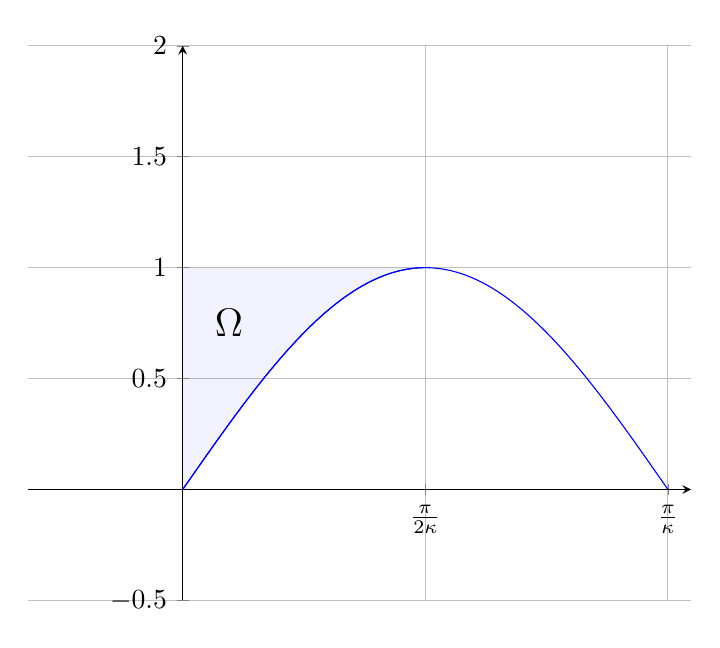
\begin{tikzpicture}
\begin{axis}[
        samples=100,grid=major,
        width=10cm,
        axis lines = middle,
        xmin=-1, xmax=pi+0.15, ymin=-0.5, ymax=2,
        restrict y to domain=0:1,
        xtick={0,1.5708,3.14159},
        xticklabels={a,$\frac{\pi}{2\kappa}$,$\frac{\pi}{\kappa}$},
    ]
    \addplot[name path=s1, domain=0:pi/2, blue] {sin(deg(x)))};
    \addplot[domain=0:pi, blue] {sin(deg(x)))};
    \path[name path=yaxis](current axis.below origin)-- (current axis.above origin);

    \addplot [
        thick,
        color=blue,
        fill=blue,
        fill opacity=0.05
    ]
    fill between[
        of=s1 and yaxis,reverse=false,
        soft clip={domain y = 0:1},
    ];
    \node [rotate=0] at (axis cs:  0.3,  .75) {\Large$\Omega$};
\end{axis}
\end{tikzpicture}

\textgreek{Οπότε: }
\begin{align*}
    &E(\Omega) = \frac{\pi}{2\kappa}\cdot1 - \int_{0}^{\frac{\pi}{2\kappa}}f(x)dx = \frac{\pi}{2\kappa}- \int_{0}^{\frac{\pi}{2\kappa}}\eta\mu(kx)dx\\
    \implies &E(\Omega) = \frac{\pi}{2\kappa} - \Big[-\frac{\sigma\nu\upsilon kx}{k}\Big]_{0}^{\frac{\pi}{2\kappa}} = \frac{\pi}{2\kappa} + \frac{\sigma\nu\upsilon (\frac{\pi}{2\kappa}\cdot\kappa)}{\kappa} - \frac{\sigma\nu\upsilon (0)}{k}\\
    \implies &E(\Omega) = \frac{\pi}{2\kappa} - \frac{1}{\kappa} = \frac{\pi-2}{2\kappa}
\end{align*}
\begin{align*}
    \lim_{\kappa\to+\infty}E(\Omega) = \lim_{\kappa\to+\infty}\frac{\pi-2}{2\kappa} = (\pi-2)\cdot 0 = 0
\end{align*}
\end{center}
    \end{questions}
\end{document}


% tkz-tab hardcodes $0$ for the zeros
%\xpatchcmd{\tkzTabLine}{$0$}{$\bullet$}{}{}
% we want solid lines
%\tikzset{t style/.style={style=solid}}
